% !TeX root = ../main.tex
% -*- coding: utf-8 -*-

\chapter{总结与展望}
\label{ch6}

综上所述,在本文的工作中我们发展了主方程--Fokker-Planck 方程的方法来描述腔磁振子系统中的量子关联。针对线性耦合模型的哈密顿量,我们得到了一组包含系统中任意阶关联函数的级联方程,并使用级联方程的特解研究了系统的稳态谱。由于腔磁振子系统的高度可调性,我们基于实验上的参数探究了强耦合,MIT,Purcell效应三种不同耦合情景下的平均粒子数与二阶关联函数稳态谱,并结合解析解理解了对应的计算结果。其中,使用平均光子数和平均磁振子数的稳态谱可以合理解释实验测量得到的稳态谱特征,而通过二阶关联函数的稳态谱我们更是揭示了系统中存在的相干竞争机制。除此之外,我们还借助随机微分方程模拟的方法研究了腔磁振子系统的动力学演化行为。在连续驱动情况下得到的结果告诉了我们系统由初态转变为稳态的详细过程,并且能够与级联方程的结果相互印证。而脉冲激励的结果在强耦合下则是呈现出和实验一致的Rabi振荡行为,与此同时受初始激励强度和温度影响的动力学演化行为也表现出相干竞争的特征。在逐渐增大系统的两种耗散率到MIT与Purcell参数的过程中,脉冲激励后的时间演化展现出了Rabi振荡削减的过程。

在我们已有的计算结果中光子的平均数(强度)和实验的特征一致,但是磁振子的平均数(强度)以及二者的二阶关联函数目前却缺乏相关的实验参考。对于磁振子的强度,目前由于实验技术的限制确实没有很好的办法去对其进行直接测量,但是对于光子的二阶关联我们还是有可用的探测手段的。
\begin{figure}[htbp]
	\centering
	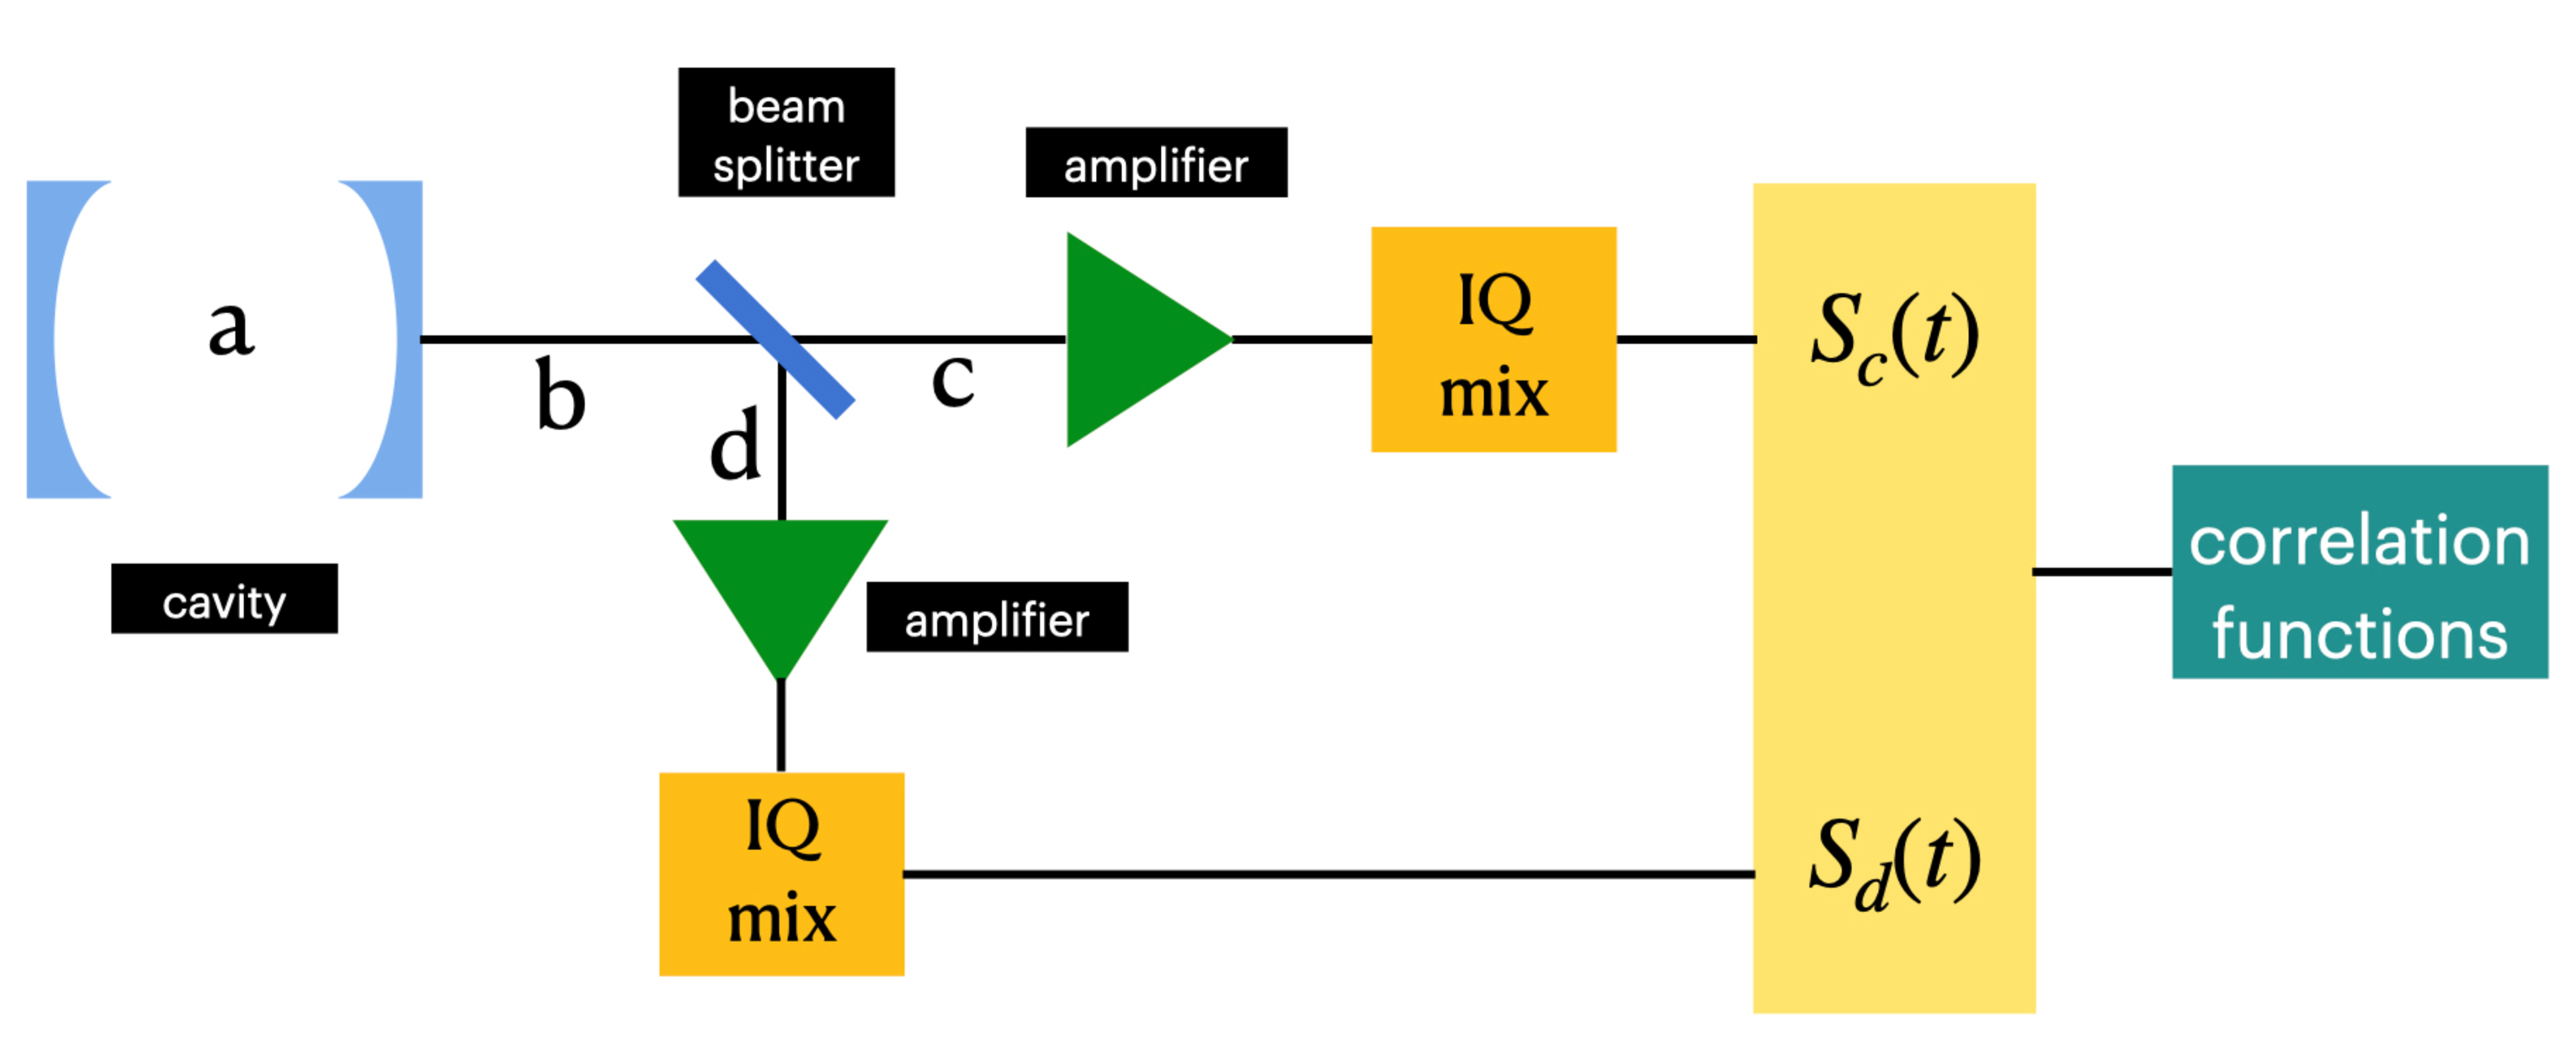
\includegraphics[width=2\basefigurewidth]{Figure6}
	\caption{测量腔中光子二阶关联的实验装置图} 
	\label{HBTExperiment}
\end{figure}
我们提出可以使用如图\ref{HBTExperiment}所示的HBT干涉实验来测量腔中光子的二阶关联。从微腔中
透射的光经过分束镜分束以及放大器放大过后,就可以对探测到的两部分光场正交量进行积分处理,从而得到光子的二阶关联,类似的实验装置已经被成功地应用于探测电路QED中的微波场,因此在腔磁振子系统中使用也是合适的。另外在我们的计算中出现的大多数参数实验上都是可以直接调节的,唯一有问题的在于脉冲激励中的相干光子数。我们在这里假设初始激励微波腔的脉冲实现方式为方波并且能量完全输入到腔体之中,方波在频率为$\omega_0=7.875$GHz的情况下持续时间为1ns,可以计算出此时$10^8$,$10^6$,$10^4$初始相干光子数分别对应于−32.8,−52.8,−72.8 dBm的方波强度。

目前的腔磁振子系统研究在室温下的实验已经有很多了,为了朝量子信息处理迈进,腔磁振子系统必须与低温下的腔QED、电路QED结合来实现对磁振子量子水平的操控。在未来的混合量子系统中,现在大量用于处理腔磁振子系统的半经典理论和量子朗之万方程的方法将不再好用,而我们使用全量子语言发展的方法就将会体现出优势来。在量子水平下出现的大量非线性效应在主方程下会表现出不同于经典的多量子涨落,而在量子朗之万方程中则不会描述这些涨落项的影响,这无疑会造成理解上的偏差。另外在磁振子系统中已经实现了超强耦合的参数,此时的耦合率大到与磁振子和腔本身的频率相当,此时的旋转波近似将不再有效,必须要改写由此导致的影响,而在主方程中可以直接将非旋转波近似的考量加入\ref{ch3}\ref{secMaster}的推导之中。总而言之,我们发展的方法具有很高的灵活性,无论未来腔磁振子系统的研究朝哪个方向发展都可以找到合适的使用机会。